\chapter{Multimodal data fusion\label{results}}

The motivation for using multiple modalities is the additional information that could be gained (\cite{8103116}). Different medical imaging methods may give more detailed information when used together, whereas tabular data may give additional information that can't be gathered from images alone. Building a machine learning model to solve a problem with data from multiple modalities eventually leads to an issue of using the different modalities together. Data fusion combines multiple modalities into a single vector or outcome, depending on the approach. One definition of data fusion is the analysis of several data sets such that different data sets can interact and inform each other (\cite{7214350}). Different diseases benefit more from certain approaches to data fusion. For example, fusion approaches that enable cross-modal interactions are essential for certain diseases, whereas others may not benefit as much from such interactions. The nature of the problem and data that is available influences the approach's effectiveness. This chapter aims to provide an overview of the common fusion architectures and difficulties associated with data fusion. Fusion strategies can be used for more than two modalities, but for minimum complexity, the approaches are presented with two modalities. Unimodal models are referred to when classifying with a single modality.

\section{Early, intermediate, and late fusion}


Early fusion is considered when the input modalities are fused into a single representation vector before feeding into the model. Early fusion uses only one model, and the difference compared to unimodal models is the input that is fused. Concatenating is one of the strategies to fuse data within early fusion (\cite{10.1093/bib/bbab569}). Concatenation of \(\vec{x} = [1, 2, 3] \text{ and } \vec{y} = [4, 5, 6],\text{ is }  \vec{x} \oplus \vec{y} = [1, 2, 3, 4, 5, 6].\) Feature extraction can help the fusing but it is seen as preprocessing not as a part of the model. Finding a common subspace for data with varying dimensions and removing correlations between modalities is important for successful early fusion (\cite{8103116}). Early fusion approaches can not propagate loss back to the original input features which is a key difference compared to intermediate fusion methods. Early fusion can utilize any supervised machine learning algorithm. Simplified architecture for an early fusion model is illustrated in \ref{fig:early_late} (a).

Using a separate model for each modality where each model outputs a prediction and combining these predictions to produce the final output is considered as late fusion. Probabilities from the independent model outputs are aggregated to produce the final output. The aggregation method varies based on the modalities and the application, for example, averaging and voting-based approaches can be used (\cite{article22}). Outputs of independent models can also be used as input to another model that makes the final prediction. Late fusion approaches make minimal use of the combined effects of modalities compared to early and intermediate approaches since each prediction is done independently. Simplified architecture for late fusion is illustrated in \ref{fig:early_late} (b).

\begin{figure}
\hfill
\subfigure[Early fusion]{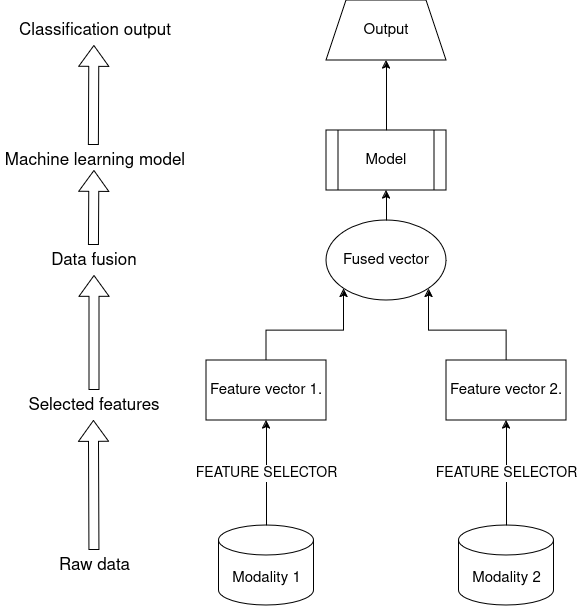
\includegraphics[width=7cm]{template/figures/Early fusion_WHITE.png}}
\hfill
\label{fig:early}
\subfigure[Late fusion]{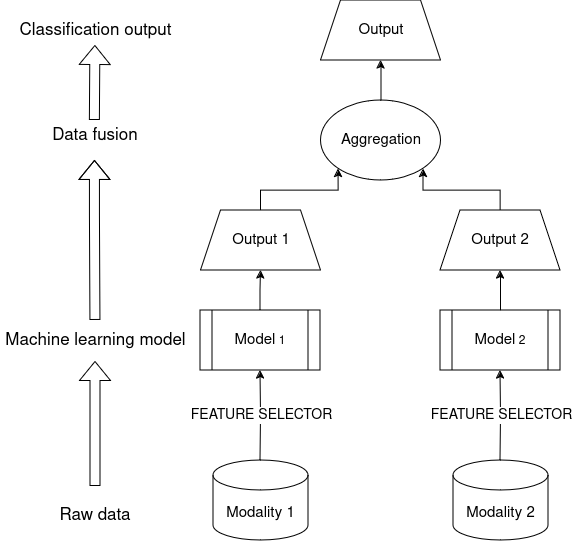
\includegraphics[width=7cm]{template/figures/LateFusion_Fwhite.png}}
\hfill
\label{fig:late}
\caption{Early and late fusion}
\label{fig:early_late}
\end{figure}

Intermediate fusion is an approach where the architecture uses multiple networks together. The model can be separated into multiple unimodal neural networks that towards the end are combined in shared layers. The input to the model is the data from the modalities and the extracted features from independent models are combined into the shared representation layer that in the end produces the output of the model. Figure \ref{fig:intermediate} shows a simplified structure of the intermediate fusion. Fusion between the modalities can also be done in different stages allowing flexibility and PCA or stacked autoencoders can be used to improve the representation in shared layers (\cite{8103116}). Using neural networks in feature extraction and after the fusion allows the loss to be propagated back to the input modality level. This allows better feature extraction since the independent models are also optimized during the training. Intermediate fusion makes use of cross-modal interactions like early fusion and modality-specific models, the same as in late fusion approaches.

\begin{figure}
    \centering
    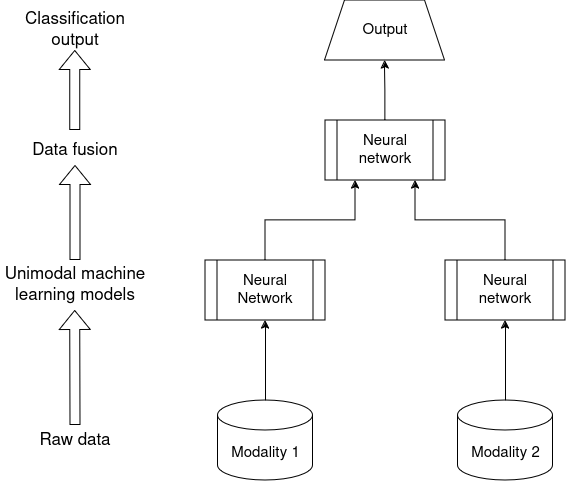
\includegraphics[width=0.5\linewidth]{template//figures/IntermediateFusion_white.png}
    \caption{Intermediate fusion}
    \label{fig:intermediate}
\end{figure}

Early, intermediate, and late fusion can be seen as the baseline for the fusion approaches. While no single approach is proven to be supreme, studies often evaluate and combine different approaches and methods suitable for the given task.
Each of the approaches has advantages and disadvantages. It have been suggested that various unimodal and multimodal approaches should be evaluated when building multimodal models (\cite{article22}), since unimodal models can be used in multimodal approaches and the most suitable fusion approach varies and depends on the problem. Considering the structure of the data fusion approaches, late fusion is suitable in situations where the modalities contain independent aspects of the data. Early fusion can make use of the cross-modal interactions. However, to make use of cross-modal interactions successfully, it might require specific preprocessing techniques. Late fusion architecture can adapt to missing modalities, offering ease when dealing with datasets where data contains different sets of modalities per sample. Independent unimodal models in the late fusion approach also offer easy addition of new modalities as the training can be done only for the additional unimodal models. Early fusion architectures may need retraining of the whole model if new modalities are added. Similarly, when the training is done with data where all modalities are present in each sample, handling missing modalities poses an issue. Relying on one model only reduces complexity compared to models relying on multiple models. Intermediate fusion offers parts from both of these with additional complexity.

Literature review reported that fusion with medical images and clinical data using multimodal fusion generally increased accuracy (1.2–27.7\%) and  Area Under Receiver Operating Characteristic Curve (AUROC\footnotemark{}) of (0.02–0.16) compared to models using a single modality for the same task (\cite{article22}). However, no single fusion strategy performed consistently optimally over all domains. In another review, multimodal data fusion was reported to increase the accuracy over unimodal approaches with a 6.4\% mean improvement in Area Under Curve (AUC\footnotemark[\value{footnote}]) (\cite{articlePreciRev}). The measurements of increased accuracy with multimodal data fusion do not mean that these models would be beneficial for clinical settings and real-world applications. End-to-end applications and prospective studies are needed to validate the relevancy of these models.

\footnotetext{AUC and AUROC are used interchangeably and noted here as they appear in the original paper. More about AUC and AUROC in \ref{appendix:sample}}

\section{Challenges with multimodal machine learning}

Challenges within multimodal machine learning have been outlined as follows (\cite{8269806}):

\textbf{1.} \textit{Representation}: how multiple modalities are meaningfully represented.

\textbf{2.} \textit{Translation}: involves the mapping of data from one modality (A) to another (B).

\textbf{3.} \textit{Alignment}: which parts of one modality directly correspond to another.

\textbf{4.} \textit{Fusion}: how to combine data from multiple modalities, particularly when some data may be missing or certain modalities are more informative than others.

\textbf{5.} \textit{Co-learning}: how to transfer knowledge between different modalities.



All of these are important technical aspects for the successful multimodal machine learning model. It is important to notice that the classification problem itself and the modalities affect heavily the issues that may arise. On top of the five key challenges related to multimodal machine learning and the context-specific ones, traditional problems in machine learning can be similarly found in multimodal architectures. 

\subsection{Explainability}

When machine learning is applied to critical fields such as medicine where the usage might have an impact directly on patient health it is crucial to have explainability on the models (\cite{article44}). Models that use deep learning are often thought of as black boxes and lack explainability. Multimodal machine learning models can have multiple of these employed. Machine learning models and especially deep learning models carry data in abstract representations that might be hard to understand. Similarly, many data fusion methods with feature extractions and shared representations hold data in abstract formats. To understand a decision that is made by the ML model additional metrics or methods can be applied. The eXplainable Artificial Intelligence (XAI) can be seen as a field that aims to produce these methods (\cite{XAI}). An example of this is seen in Shapley values that have been used for measuring the contribution from different modalities (\cite{articlehaim}). Explainability and justification of classification decisions in the models utilized is one of the key challenges to when machine learning models are utilized in medical context. 

\subsection{Data in medical context}

The medical field offers vast amounts of datasets that derive from retrospective studies. Biobanks, national registries, and open-source datasets are sources of data in multimodal medical studies. Datasets such as MIMIC (\cite{articlemimic4}) that are open source are used as a benchmark to compare models. The prospective studies to validate models built with retrospective data are an important part of understanding the true utility and real-world performance of these systems (\cite{kelly2019key}). A specific dataset is needed to apply multimodal machine learning to certain diseases. Privacy in the medical context also limits the data available. In a recent review, small sample sizes and imbalanced samples were reported as common limitations to studies employing multimodal machine learning models (\cite{articlePreciRev}). Small sample sizes and high dimensionality combined increase the sparsity of the data which can also lead to a curse of dimensionality (\cite{articlecurse}). The curse of dimensionality appears in problems like overfitting. While the curse of dimensionality and various problems associated with are well-known in machine learning, assessing them is a necessary step when building multimodal machine learning models. Choosing the correct architecture is an essential part of building a multimodal machine-learning model. Comprehensive evaluation requires the building of multiple models. Conducting high-quality research in this area can be challenging because it involves complex computational models, requires validation studies, and needs expertise from various fields.
